
\chapter{A New Paradigm for Model Individualization in T1DM}
\label{sec:InSilicoIdentification}

All the mathematical models for T1DM reviewed in this thesis suffer from problems that lead to not mimicking the real patient's physiology. Virtual patient's identification is defined as an identification procedure analog to the experimental data fitting, where the virtual data are generated with the same model used for identification. Uncertainty can be then artificially added to the virtual patient's data to challenge the identification method. The aim of this experiment is to test the methodology of identification in the diabetes context.

Interval models were used for consideration of uncertainty within the diabetic patient, and for the identification fitting. Virtual patients were simulated with inherent variations in their physiologic parameters in order to simulate intra-patient variability. Interval bounding of all the possible outputs of the patients has to be performed for the complete characterization of the patient's data, but overestimation of the uncertainty has to be considered and penalized when using interval models for identification.  From this point of view, we devised another point of view to interval identification. In this thesis, dual objective minimization is used to accomplish interval identification of diabetic patients. the two objectives to be optimized are: 1) the interval data bounding, 2) the glucose interval width. Both objectives are competing in the sense that maximizing the interval output of the model surely will bound more data samples, but the prediction capabilities of the model are worsened.

Multiobjective optimization was then applied to both simulated gold reference data and simulated CGM data of the same patient's, and the results compared.

\section{Optimization Set-up}
\label{sec:MultiobjectiveOptimizationSetUp}

Classic parametric identification results in a single point in the parameter space, being insufficient for the case of a time-varying model based on poor prediction capabilities. Bounding all glucose measurements by means of an interval model, with time-varying parameters considered as intervals, may help identifying both the patient and the intra-patient variability, increasing the robustness of the derived therapies or control algorithms. However, in the case of home monitoring where large measurement errors may appear (especially due to CGM) some relaxation may be needed to avoid large intervals for parameters that loosely fit the physiological variability. 

Identification of interval models has been traditionally addressed under the framework of bounded-error identification (see Chapter \ref{sec:ErrorBoundedEstimation} and references therein). However, when large intra-patient variability is present no parameter values consistent with the error will generally be found. Robust predictions for therapeutic decisions can be achieved if the interval model is able to bound the patient's response, i.e., the experimental measurements should be included in the output envelope predicted by the model at each time instant $t_i$

\begin{equation}
y^{\ast}(t_i) \in y(t_i ;\mathbb{P}), \;\;\; \forall i \in I
\label{eq:measurementscontained}
\end{equation}
	
where $y(t_i ;\mathbb{P})=[\underline{y(t_i ;\mathbb{P}}),\overline{y(t_i ;\mathbb{P})}]$ stands for the interval prediction at time instant $t_i$ for the to-be-identified parameter set $\mathbb{P}$ and $I=\left\{1,...,n\right\}$ is the index set of the available measurements. In practice, a relaxation of the above problem may be needed, allowing for small errors with respect to the inclusion envelope due to noise in the measurements and compensation for non-modeled dynamics. 

Interval parameter values $\mathbb{P}$ must be found so that the model output envelope bounds the measurements. Denoting as $G^{\ast}(t_i)$ the glucose measurement at time instant $i$, equation \eqref{eq:measurementscontained} can be rephrased as:

\begin{equation}
G^{\ast}(t_i) \in [\underline{G(t_i;\mathbb{P})},\overline{G(t_i;\mathbb{P})}], \;\;\; \forall i \in I
\label{eq:measurementscontained2}
\end{equation}

where $\underline{G(t_i;\mathbb{P})}$ and $\overline{G(t_i;\mathbb{P})}$ (onward $\underline{G}$ and $\overline{G}$) are the lower and upper bounds of the glucose interval $\boldsymbol{G}$.

\begin{figure}[hbtp]
\centering
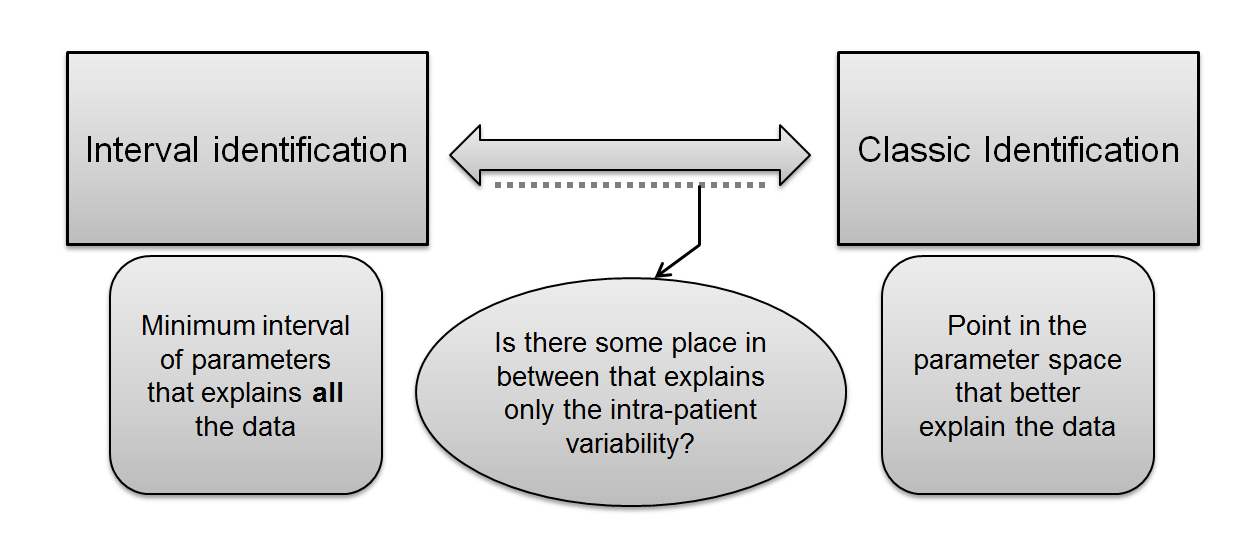
\epsfig{file=Figures/espectro.png, width=\textwidth}\caption{Ranging from classic to interval identification.}
\label{fig:espectro}
\end{figure}

In Figure \ref{fig:espectro} a possibility of hybrid identification ranging form classic to interval is hinted. Given the fact that neither the classic identification point of view is valid for the current diabetic patient models (due to parameter variability), and also considering that the pure interval bounding is inefficient due to large measuring errors, a compromise is required for the appropriate characterization of real patient variability. The hypothetical trade-off point in between the two identification paradigms has never been investigated in literature (to my knowledge). Should this point exist, the compromise errors that are derived from this methodology will be characterized in the following lines.

Multi-objective identification is the process of simultaneously optimizing two or more conflicting objectives subject to certain constraints. The solution of this kind of problems is not a single optimal point in the objectives search space, but a family of solutions called a Pareto Front (PF). Each individual in the family is non-dominated by the other individuals, i.e. they cannot be replaced by other point in the objective space for improving an objective, without worsening another one. Evolutionary algorithms are popular solvers for this kind of problems. The $\epsilon$-MOGA evolutionary algorithm \cite{herrero2007well} was used in this work.

Optimization requires the objectives to be defined as minimization indexes. The first objective considered for minimization of the fitting error. The error was computed here as the sum of squares of the Hausdorff distance $d_H$ between the samples and the predicted envelope: 

	\begin{gather}
	J_e(\mathbb{P}):=\sum\limits_{i=1}^n d_H^2 \left( G^{\ast}(t_i), \boldsymbol{G} \right) \label{eq:jota1} \\
	d_H \left( G^{\ast}(t_i), \boldsymbol{G} \right):=
	\begin{cases}
	0 & \text{if} \; G^{\ast}(t_i) \in \boldsymbol{G} \\
	G^{\ast}(t_i)-\overline{G}  & \text{if} \; G^{\ast}(t_i) > \overline{G}  \\
	\underline{G} -G^{\ast}(t_i) & \text{if} \; G^{\ast}(t_i) < \overline{G} 
	\label{eq:jota12}
	\end{cases}
	\end{gather}

where $i$ denotes the sample index, $n$ is the number of measurements, $G^{\ast}(t_i)$ the $i$-th glucose measurement and $ \boldsymbol{G} := \left[ \underline{G},\overline{G} \right]$ the glucose interval predicted for time sample $i$ given by the interval model. This is computed by means of a guaranteed interval simulator as proposed in \cite{calm2010comparison}. Thus, if $\left| \overline{G} - \underline{G} \right| = 0 $ (null interval width) then $J_e$ corresponds to the classic sum-of-squares cost index. If $J_e=0$, the envelope given by $[\underline{G},\overline{G}]$, encloses all the measurements. 

The other objective, by definition of multi-objective optimization, must be conflicting with the first one in the minimization. Given that when working with intervals the error is minimized by simply increasing the size of the interval (trivial solution at maximum width), the other objective to be pursued must be a minimization of the interval width. The following index is then considered:
	\begin{equation}
	J_w(\mathbb{P}):=\max_{i \in I}\left( \text{width} \left( \boldsymbol{G} \right) \right) = \max_{i \in I} \left( \overline{G}- \underline{G}\right)
	\label{eq:jota2}
	\end{equation}	
Maximum width was chosen for the minimization because variability in the width of an interval model response can be very high in the postprandial period. Minimizing average widths for example may lead to very wide glucose intervals in the early postprandial period which translate in wide interval parameters. Instead, limiting the maximum width narrows the interval more consistently throughout all the postprandial period.

Both objectives can be shown in a cartesian plot, in order to visually characterize the PF. An example of a PF is shown in Figure \ref{fig:paretoYSI}. The extremes of the PF correspond to the classic (right) and interval approach (left). In between, every point in the PF is a relaxation of the interval approach. 

\begin{figure}[hbt]
\centering
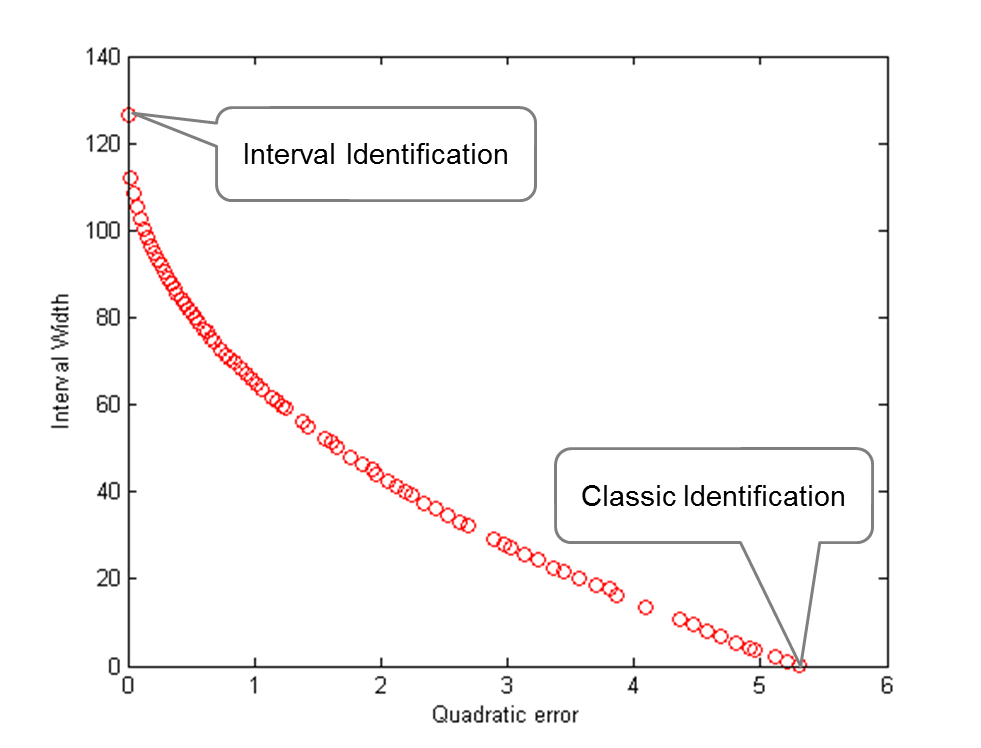
\epsfig{file=Figures/paretoYSI.png, width=0.9\textwidth}\caption{Example of a Pareto Front exploring all optimal possibilities from a zero-width problem (classic identification) to a minimum-width problem with zero error (interval approach).}
\label{fig:paretoYSI}
\end{figure}

The selection of the ``best'' solution in the PF will depend on the nature of the measurements and the desired degree of robustness. When using reliable measurements (e.g. reference BG measured with a YSI 2300 STAT Plus\texttrademark{} Glucose Analyzer), and assuming there is no model mismatch, it is desired that all the data points are predicted by the glucose envelope generated by the model, i.e. $J_e=0$. This is equivalent to choosing the pure interval solution of the problem. 

As already said, identifying with CGM data is much more challenging due to the accuracy limitation of these devices, but home monitoring is undoubtedly more feasible for clinical practice. The optimization method works the same way independently of the data source, but choosing one point or another in the PF does not. The zero-error solution only makes sense when identifying from reference BG since it encloses robustly all the data available, which are reliable. When CGM is used, data cannot be trusted as much as reference BG, so a tradeoff solution has to be chosen.

A relaxation is thus needed in order to identify an interval model representing actual patient's variability. Two solutions can be devised: 
\begin{itemize}
	\item Choosing an ``acceptable'' error, and finding the closest PF individual for that error.
	\item Estimating an appropriate maximum width for the glucose envelope, and choosing a PF individual accordingly.
\end{itemize}

The second approach is used here. Indeed, the optimal width of the pure interval solution for the BG-based identification may be a good approximation of intra-patient variability. Thus, a method is needed to estimate this optimal width from CGM data. This is explored further in later sections of this chapter.

Even though identification in a domiciliary environment can only be performed reasonably with a CGM, reference BG is the variable that the model attempts to predict, and as such it is the signal to be used for the validation of the identifications performed. In order to calculate the prediction abilities of the identified model, the Mean Absolute Relative Error referred to a glucose envelope ($MARD_I$) was used:
\begin{align}
	MARD_I[\%] &:= \frac{\sum\limits_{i=1}^n\left|\frac{d_H\left(BG_i, \boldsymbol{G}\right)}{BG_i}\right|\ast 100}{n} \label{eq:mardi} \\
	d_H\left(BG_i, \boldsymbol{G}\right) := &
	\begin{cases}
	0 & \text{if} \; BG_i \in \boldsymbol{G} \\
	BG_i - \overline{G} & \text{if} \; BG_i > \overline{G} \\
  \underline{G} - BG_i & \text{if} \; BG_i < \underline{G}
	\end{cases}	
\end{align}
where $BG_i$ is the reference BG measurement at time $i$, $n$ is the number of data points, and $d_H$ is the Hausdorff distance from the point $BG_i$ to the interval $\boldsymbol{G}$ representing the glucose envelope at time $i$ given by the interval model.  

All statistical significances were calculated using Student's t-test for the correlation values.
	
\section{Identification from reference glucose}
\label{sec:IdentificationFromReferenceGlucose}

A cohort of 14 virtual patients was generated by means of the Cambridge's model. Three postprandial periods were simulated for each patient, according to the optimal experiment design described in Chapter \ref{sec:OptimalDesign}: on Day 1 and Day 3 a meal with 100 grams of carbohydrates (CHO) was ingested and the insulin bolus was advanced 30 minutes; on Day 2 the patient ate a 40-gram CHO meal and delayed the bolus for 120 minutes. For all simulated days the patient was considered at euglycaemic before the meal intake (model initial conditions). This experimental set-up was shown to be beneficial for model identification due to the separation of insulin and meal dynamics.

The virtual patients were considered to have intra-patient variability (time-varying model parameters). Input errors were also considered for the insulin infusion rate and the estimation of carbohydrate intake. The parameters considered time-varying are listed next:
\begin{itemize}
	\item $S_{iT}$: insulin sensitivity on glucose transport from blood to interstitium.
	\item $S_{iD}$: insulin sensitivity on glucose utilization.
	\item $S_{iE}$: insulin sensitivity on endogenous glucose production.
	\item $k_e$: insulin elimination rate.
	\item $k_{12}$: rate of glucose transport from interstitium to blood.
\end{itemize}
Given that the uncertainty in the meal and insulin subsystems was considered in artificial aggregated parameters (described later), the following parameters were treated as patient-dependent and time-invariant:
\begin{itemize}
	\item $t_{maxG}$: time constant for glucose absorption in the gut.
	\item $t_{maxI}$: time constant for insulin absorption.
\end{itemize}
Additionally, the following input errors were introduced:
\begin{itemize}
	\item $\beta$: a random time-varying error for the insulin infusion rate from the insulin pump.
	\item $\alpha$ estimation: a repeated bias plus a random time-varying error for the carbohydrates estimation given by the patient. 
\end{itemize}

The identification algorithm considered that every uncertain parameter was characterized by its lower and upper bounds. The final parameter identification vector results:
\begin{equation}\label{eq:parametervector}
%\begin{split}
\theta=[ \underline{S_{iT}}, \overline{S_{iT}}, \underline{S_{iD}}, \overline{S_{iD}}, \underline{S_{iE}}, \overline{S_{iE}}, \underline{k_{12}}, \overline{k_{12}}, \underline{k_e}, \overline{k_e}, \underline{\alpha}, \overline{\alpha}, \underline{\beta}, \overline{\beta}, t_{maxI}, t_{maxG} ]
%\end{split}
\end{equation}
where $\underline{S_{iT}}, \overline{S_{iT}}$ are the lower and upper bounds of the parameter $\boldsymbol{S_{iT}}$. Similar notation is used for the rest of the interval parameters. $\boldsymbol{\beta}$ and $\boldsymbol{\alpha}$ stand for errors in pump infusion and meal estimation respectively. $t_{maxI}$ and $t_{maxG}$ are the only real-valued parameters.

Variability in the meal absorption is characterized by uncertainty in the meal estimation and variability in insulin pharmacokinetics is characterized by the parameter $k_{e}$ and uncertainty in the insulin pump infusion. For the sake of simplicity, the time-varying parameters and errors considered were assumed constant throughout a postprandial period for the virtual data generation. However, they were changed from one day to another of monitoring following a random process with mean equal to the nominal value of the parameter (0 for the errors) and a standard deviation of 10\% of the nominal value. As demonstrated by Calm \textit{et al.} \cite{calm2007prediction} using optimal interval simulation methods, the consideration of 10\% uncertainty in the model parameters may produce glucose trajectories differing in 100 mg/dL, so it is considered a sensible value for the reproduction of variability.

When interval parameters are considered, the simulation of the model must produce a glucose envelope representing the set of possible glucose trajectories that the patient may exhibit according to the defined intra-patient variability. To this end, the interval simulators for the Cambridge model developed in \cite{calm2010comparison} and \cite{de2012prediction} were used in this work.

Measurement errors induced by a CGM device during home-monitoring were simulated. In this work the model presented in Chapter \ref{sec:CGMStatisticalModelingAndValidation} was used for simulation of the real-time CGM Dexcom\textsuperscript{\textregistered} SEVEN\textsuperscript{\textregistered} PLUS (Dexcom\textsuperscript{\textregistered}, San Diego, CA), due to more accurate modeling results produced. 

An example of identification for one representative patient is shown in Figure \ref{fig:classicvsintervalYSI}. This patient is an illustrative example, but little differences are found from one patient to another. For this patient two simulations, corresponding to both ends of the PF in Figure \ref{fig:paretoYSI}, plus the BG data are plotted. As expected, the output of the interval model robustly encloses all the simulated days, successfully finding the global minimum of the interval identification problem.
\begin{figure}[hbt]
\centering
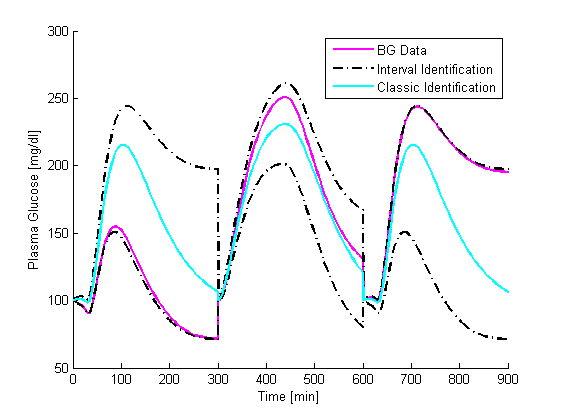
\epsfig{file=Figures/classicvsintervalYSI.png, width=0.9\textwidth}\caption{Comparison of classic and interval identification. Three 5-hour postprandial periods in consecutive days are shown. The first and third days correspond to identical meals and insulin infusion. Black dotted lines represent the interval solution, enclosing all the monitoring days. The cyan line (classic identification) behaves as an average glucose profile for the three days.}
\label{fig:classicvsintervalYSI}
\end{figure}
As for the rest of the patients, the identified interval models covered completely the data for all the postprandial periods. As expected, the method does not encounter any difficulty on reproducing noise-free data. However, identification from BG reference data is very limited due to the requirement of in-patient studies. Further investigation is required on the presence of uncertainty in the measurements introduced by CGM.

The pure interval extreme of the PF is in the following considered the real variability of each patient, and the width associated (error is zero for all cases) is considered the optimal width to be identified in each case.

\section{Identification from CGM}
\label{sec:IdentificationFromCGM}

Figure \ref{fig:YSIvsCGMpareto} shows the BG-based and CGM-based Pareto Fronts for the sample patient. For the same error, all the models identified from the CGM have wider intervals than the ones from reference BG. This is also true in the rest of the patients, especially as it gets closer to the pure interval solution (zero error). 
\begin{figure}[hbt]
\centering
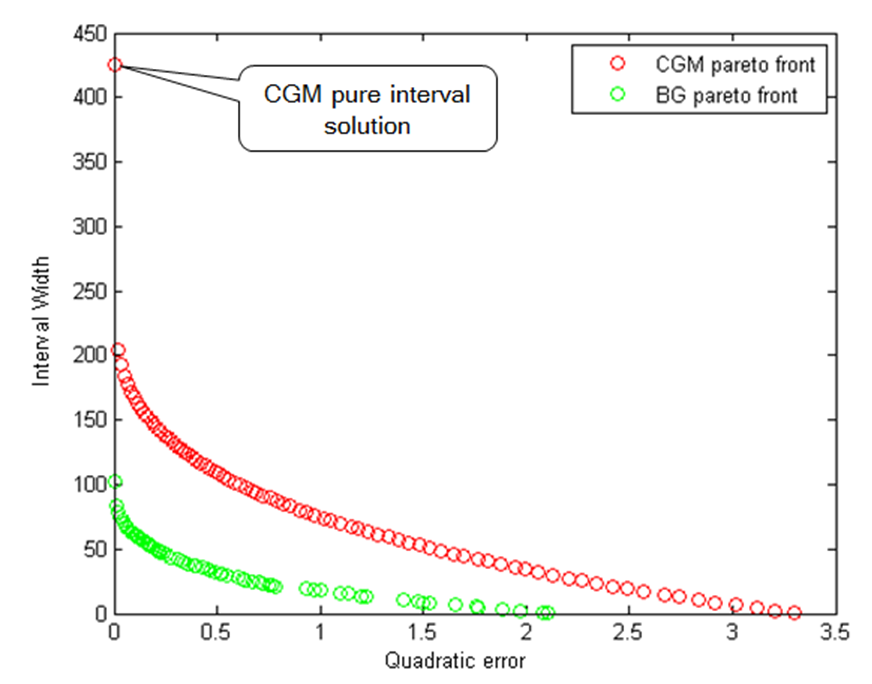
\epsfig{file=Figures/YSIvsCGMpareto.png, width=\textwidth}\caption{Both PF for the identification of a patient, using CGM and BG data. CGM identification shows larger width and error for most patients. CGM pure interval identification requires too wide prediction envelopes.}
\label{fig:YSIvsCGMpareto}
\end{figure}
The top left solution in the PF for CGM identification has a much larger width that any other individual in the solution. Such a large width is necessary to cover all the CGM excursions especially due to the error present in the first time instants of every postprandial period, where the glucose envelope given by the model is very thin, but the CGM measurements may be very noisy. From a practical point of view this solution can be discarded.

The CGM-based identification results for both ends of the PF are shown in Figure \ref{fig:classicvsintervalCGM}. As with the glucose reference fitting, classic identification shows only an average behavior. The interval model covers all the data provided by the CGM but patient's actual intra-patient variability is overestimated since it is confounded by CGM measurement error. 
\begin{figure}[hbt]
\centering
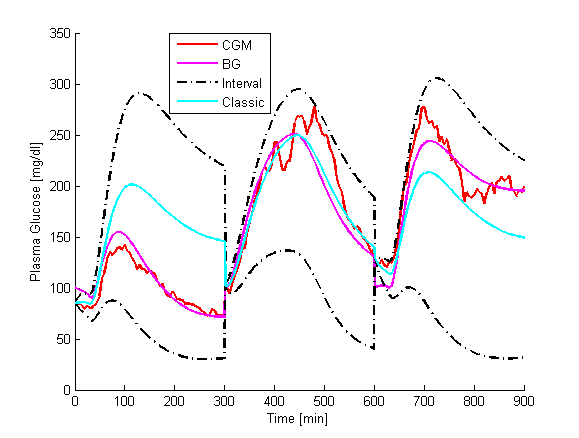
\epsfig{file=Figures/classicvsintervalCGM.png, width=\textwidth}\caption{Comparison of classic and interval identification from CGM. Black dotted lines are too wide to be considered useful. Three 5-hour postprandial periods in consecutive days are shown. The first and third days correspond to the same meal and insulin infusion to the patient.}
\label{fig:classicvsintervalCGM}
\end{figure}
As stated earlier, a method for estimation of the ``optimal width'' (width for pure interval identification on BG data) for each patient is needed. Correlation between the optimal width and the so-called ``experimental width'' obtained from the overlapping of responses for similar days was investigated. Experimental data was used to further understand correlations between BG and CGM widths in real patients. The possibility of estimating the BG-based experimental width from the CGM signal, and thus the optimal width for the identification, was investigated with the analysis of clinical data from 12 patients who underwent clinical mixed meal studies as described in detail in \cite{paoloibolus2012}. Postprandial variability was analyzed after two predetermined meals containing 40 g or 100 g of carbohydrates with normalized initial conditions through an insulin feedback procedure. Each patient was evaluated in 4 different occasions, twice with each meal. Frequent YSI measurements were taken simultaneously to a Dexcom\textsuperscript{\textregistered} SEVEN\textsuperscript{\textregistered} PLUS monitor. The BG-based optimal maximum width is highly correlated to the maximum width observed by overlapping the BG signal (experimental width) for days 1 and 3 where the patient ate the same meal (r=0.848,p<0.005). This is also true for the average width for all the days of the postprandial period (r=0.797,p<0.005).

In practice neither the optimal width nor the possibility of overlapping several BG postprandial periods is available. To cope with this, experimental correlations between BG and CGM width were investigated using the experimental dataset introduced before. Table \ref{tab:widthscorre} shows the results obtained demonstrating the existence of high correlation between the CGM-based and the BG-based width computations from the experimental cohort. Table \ref{tab:widthscorre} also shows the correlation among the BG-based and CGM-based widths for an \textit{in silico} study with the virtual patients' cohort reproducing the clinical study design in \cite{paoloibolus2012}. Correlations are very similar, reinforcing the CGM model used and the findings of Chapter \ref{sec:CGMStatisticalModelingAndValidation}.

\begin{table}[hbtp]
	\centering
	\begin{tabular}{ c  c | c  c }
	\hline 
	 & & \multicolumn{2}{c}{CGM} \\
   & & Max width & Avg width  \\
	\hline 
  \multirow{2}{*}{BG} & Max width & 0.67 (0.72) & 0.75 (0.66) \\
	& Avg width & 0.79 (0.87) & 0.86 (0.88) \\
	\hline 
	\end{tabular}
\caption{Correlations of postprandial BG-based vs. CGM-based widths for the experimental patients' cohort. The \textit{in silico} counterparts of the same correlations are shown within parenthesis.}
\label{tab:widthscorre}
\end{table}

Table \ref{tab:optwidthestimators} shows the correlations of the BG-based optimal width (both maximum and average) with the experimental width from the CGM. These correlations were found on the virtual patients' cohort. Out of the three days of monitoring, maximum and average widths of CGM overlapping signals are studied as estimators for the optimal width found in the identification from reference glucose. Max3 and Avg3 are the maximum and average width from the three days of the experiment, respectively. Max2 and Avg2 correspond to the maximum and average width from 2 equal days (days 1 and 3), respectively.

\begin{table}[hbtp]
	\centering
	\begin{tabular}{ c  c  c  c  c }
	\hline 
	 & \multicolumn{4}{c}{CGM experimental width} \\
   & Max3 & Avg3 & Max2 & Avg2 \\
	\hline 
  Optimal maximum width & 0.565 & 0.781 & 0.775 & \textbf{0.832} \\
	Optimal average width & 0.588 & \textbf{0.8} & 0.707 & 0.78 \\
	\hline 
	\end{tabular}
\caption{Correlations of optimal widths in the virtual patients vs. CGM model-based experimental widths. The best estimators (best correlations) of optimal widths are highlighted.}
\label{tab:optwidthestimators}
\end{table}

All correlations shown in Table \ref{tab:optwidthestimators} are significant (p<0.005). The best correlations are obtained for the average CGM experimental width, either for 3 or 2 days. This better correlation is due to the influence of the averaging computation in the CGM noise, which is alleviated throughout the postprandial period. The corresponding regression lines to both estimators corresponding to the average of CGM signals are:
\begin{align}
	OptimalMaxWidth =0.6617 \ast Avg2+60.4569 \label{eq:OptimalMaxWidth} \\
	OptimalAvgWidth =0.3979 \ast Avg3+27.2764 \label{eq:OptimalAvgWidth}
\end{align}
Finally, equation \eqref{eq:OptimalMaxWidth} or \eqref{eq:OptimalAvgWidth} will define the individual in the CGM-based PF to be chosen as optimal identification. This is equivalent to launching a constrained optimization problem with $J_1$ as cost index and fixed glucose envelope maximum width given by \eqref{eq:OptimalMaxWidth} or fixed average width given by \eqref{eq:OptimalAvgWidth}. This sort of optimization should then include non-linear constraints on the output of the optimization model, which may be difficult depending on the optimization algorithm.

As an illustration, the identification results for the sample patient are shown in Figure \ref{fig:comparewidthestimators}, where Avg2 and Avg3 estimators are compared. The use of CGM experimental widths over a number of days for predicting the ``optimal'' width of a particular patient is then justified. However, the predictive capability of the identified model is still to be checked. 

\begin{figure}[hbtp]
\centering
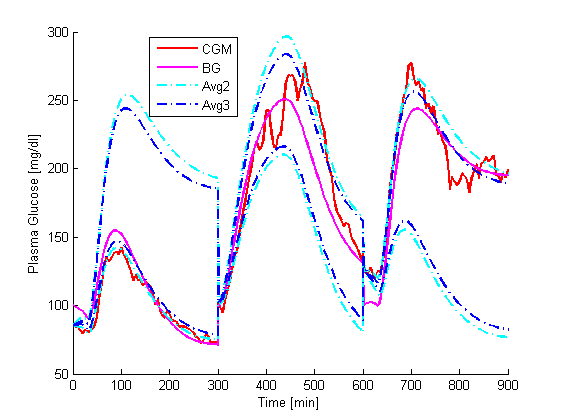
\epsfig{file=Figures/comparewidthestimators.png, width=\textwidth}\caption{Comparison of Avg2 and Avg3 estimators for the optimal width in the identification from CGM data. There is little difference between estimators, but there is a big difference between the use of optimal width estimation and pure interval identification from CGM data (see figure \ref{fig:classicvsintervalCGM}). Three 5-hour postprandial periods in consecutive days are shown. The first and third days correspond to the same meal and insulin infusion to the patient.}
\label{fig:comparewidthestimators}
\end{figure}

Results of the BG prediction errors are shown in Table \ref{tab:valestimators} for the virtual patients' cohort. The mean error for the samples not enclosed by the glucose envelope ($d_H$>0) is also computed for comparison purposes, and denoted as $ErrOut$. In order, the table shows the median for the population of the estimated width, the number of samples enclosed in the glucose envelope, the relative error considering only the samples outside the glucose envelope, and the $MARD_I$ (\%). The two width estimators that showed better correlations, as highlighted in Table \ref{tab:optwidthestimators}, were tested.

\begin{table}[hbtp]
	\centering
	\begin{tabular}{ c  c  c  c  c }
	\hline 
	 & \multicolumn{4}{c}{Avg2} \\
   & $MaxWidth [mg/dL]$ & $Predicted [\%]$ & $ErrOut [\%]$ & $MARD_I [\%]$\\
	Median & 83.3 & 67.8 & 7.5 & 3.3\\
	Min/Max & 67.6/163.3 & 34.3/97.9 & 1.9/38.3 & 0.1/11.9\\
	\hline 
	 & \multicolumn{4}{c}{Avg3} \\
  Median & 61.4 & 52.8 & 8.3 & 4.6\\
	Min/Max & 42.4/96.4 & 35/97.9 & 2.4/30.9 & 0.1/15.6\\
	\hline 
	\end{tabular}
\caption{Widths and prediction errors for the selected (best) optimal width estimators. Top row shows the performance of the identification if the maximum glucose envelope width for each patient is predicted from the width of two identical days. Bottom row displays the case when the average glucose envelope width for each patient is estimated from the width if the 3-day CGM registries.}
\label{tab:valestimators}
\end{table}

A long-term simulation of a 15-day monitoring period for a sample patient was analyzed in order to test the method's strength when coping with longer monitoring periods and outliers. The same procedure described before for virtual patient data generation was used for the generation of this dataset. In this case a total of 7 meals with 40-gram CHO content and 8 meals with 100-gram CHO content were given as input to the model. Variability of the uncertain parameters remained at 10\% of the nominal value of the parameters.

Visual representation of four out of the 15 simulated days are shown in Figure \ref{fig:15days_4days_extract}. Optimal width (computed from BG-based model identification) is compared against Avg3 width estimator, consisting in equation \eqref{eq:OptimalAvgWidth} applied to the average width of the 15-day simulation. The four days selected represent ``worst-case'' results and illustrate the performance of the method against large CGM measurement error (days 1, 3 and 15) and outlier patient behavior (day 11). For the rest of days similar results than those shown in Figure \ref{fig:comparewidthestimators} were obtained. 

\begin{figure}[hbtp]
\centering
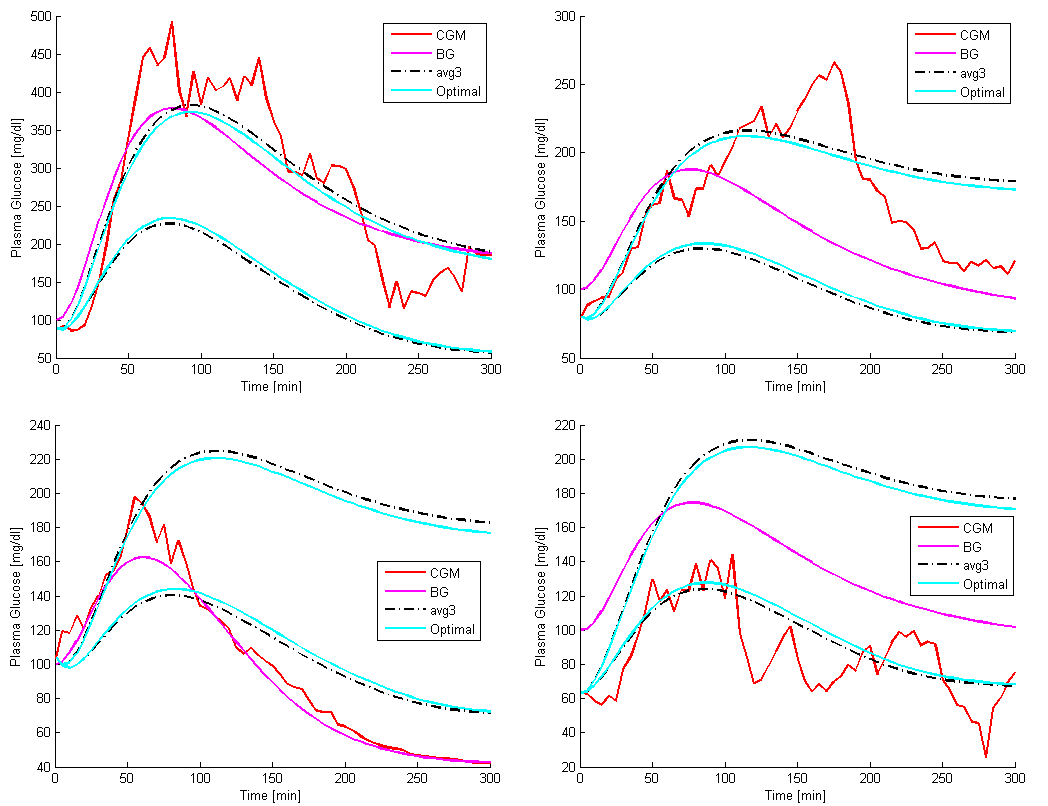
\epsfig{file=Figures/15days_4days_extract.png, width=\textwidth}\caption{Comparison of Avg3 width estimator and the optimal width for the 15-day identification experiment. Top right (Day 1), top left (Day 3) and bottom right (Day 15) panels show cases of CGM monitoring errors with satisfactory BG prediction from the model. The bottom left panel (Day 11) shows the only case where BG was not enclosed by the predicted glucose envelope for most part of the postprandial period due to the outlier patient behavior (extreme parameter values).}
\label{fig:15days_4days_extract}
\end{figure}

Reviewing the characteristics of the outlier day from the 15-day simulation, a special combination of glucose lowering power is hinted, which seems not to be present in any other day of the experiment. To check this, Figure \ref{fig:parametersperdaystack} shows the variation of the most relevant parameters for each simulated day in the 15-day experiment. Only the insulin-related parameters are displayed for the sake of clarity even though parameters were subject to variability as stated earlier. In the figure, variation is calculated as relative to the nominal parameter, and it is considered positive if it induces a decrement of glucose concentration (e.g. larger insulin sensitivities), and negative if it causes glucose to increase (e.g. larger insulin elimination rate). Displaying the parameters deviation in a stacked form as in Figure \ref{fig:parametersperdaystack} provides helpful information on the final influence of variability on the model's output for a particular day. However, variation magnitude does not directly correlate to the magnitude of the effect since not all the model parameters have the same sensitivity.

\begin{figure}[hbtp]
\centering
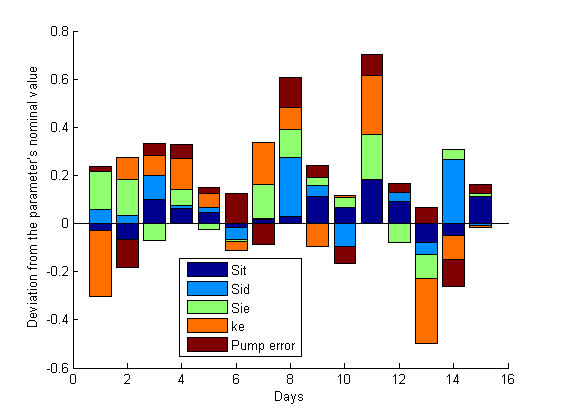
\epsfig{file=Figures/parametersperdaystack.png, width=\textwidth}\caption{Depiction of the parameter variation within the 15-days experiment. For the sake of simplicity, only the insulin-related parameters are shown here. Parameter deviation is positive if it produces a decrement of glucose levels and negative otherwise.}
\label{fig:parametersperdaystack}
\end{figure}

\section{Discussion}
\label{sec:Discussion}

Identification from virtual data supposes a much lighter challenge than experimental identification, but very interesting findings are extracted from this chapter, considered as the basic previous work before facing the problems of experimental data management.
	
The identification from reference BG data was successful, as illustrated in Figure \ref{fig:classicvsintervalYSI}. The identified interval model was able to capture patient's variability with minimum width when no measurement error is present in the data. Day 1 and day 3 correspond to the same meal, but patient's behavior is very different, as typically observed in the clinical experience. Nonetheless, the model was able to capture this variability. It is likely that the use of interval models may help in deriving more robust glycaemic control strategies.

Width estimation prior to identification is required for CGM-based identifications. Very strong correlations were found between the experimental widths from reference glucose and CGM data for real type 1 diabetic patients. Therefore the estimation of the optimal width from CGM measurements seems feasible. The maximum correlation was obtained among average widths, as illustrated in Table \ref{tab:widthscorre}. Very similar correlations were calculated for the virtual patient cohort, encouraging the use of the CGM model proposed. As Table \ref{tab:optwidthestimators} shows, the average widths of the overlapped patient's CGM postprandial traces were better correlated and thus they were better estimators of the optimal width of each patient. This may be due to the fact that averaging CGM widths can filter outliers in the CGM signal width, while maximum width values do not. Noisy outliers in the CGM signal width do not correlate well with BG widths, which are considered to be noise-free. Note that Avg2 computes the average from two identical days while the optimal average width corresponds to the whole identification period so they are not directly comparable. Finally, the optimal width estimation was computed from virtual CGM data from successive days using linear regression models.
 
Overlapping of two identical days (Max2 and Avg2) yielded much better estimations of the patient's optimal width, as data in Table \ref{tab:optwidthestimators} shows. This can be explained by the fact that the glucose variability observed in two days with the same meal and insulin therapy is a more accurate description of the patient's physiological variability, since there is no uncertainty in the model inputs. In future data acquisition experiments, repeating of identical days should be a priority. In reality though, obtaining two identical monitoring days for a patient can be very difficult. So, two different optimal width estimation methods were provided giving more flexibility independently of the data available.

The validation of the model and its prediction ability was satisfactory, as shown in Table \ref{tab:valestimators}. The model was able to predict about 60\% of the reference samples in the postprandial period, with a slightly better performance of Avg2 estimator. The non-predicted samples showed relative errors below 10\% in both cases. Regarding $MARD_I$ an error below 5\% was obtained. Thus, the proposed method allows identifying satisfactorily interval models characterizing intra-patient variability from CGM data. 

Regarding the 15-day simulation study, all the simulated days were well predicted within the model's boundaries except day 11 (see Figure \ref{fig:15days_4days_extract}), despite the error introduced by considering the CGM measurement as initial condition at each postprandial period. Day 11 gathers several factors that make it very difficult to predict.  As shown in Figure \ref{fig:parametersperdaystack}, at day 11 all the parameters pulling glucose concentration down to hypoglycemic range concur with maximum values, i.e., it can be considered an outlier behavior. This is likely to happen in rather large experiments, where extreme variability at particular days may be found. Unfortunately, outlier behavior is unpredictable, and cannot be separated in the identification process from CGM malfunctions, which are much more common. 

As shown in Figure \ref{fig:15days_4days_extract}, days 1, 3 and 15 are a good representation of the ability of the model to filter CGM malfunctions. On days 1 and 3 the monitor glucose readings were larger than reference glucose, at the risk of overestimating the glucose envelope width during the identification process. However, optimal width estimators are able to cope with this problem successfully predicting the actual BG values without width overestimation. Similarly, BG at day 15 was greatly underestimated by the CGM for the whole postprandial period. Nonetheless, this did not affect the predicted glucose envelope, which successfully enclosed BG except for the effect of the error in the initial conditions. It is deduced that the method is robust when confronted to outliers. Good prediction in most days of monitoring is achieved even in presence of extreme patient variability (day 11) or CGM malfunctions (days 1 and 15). 

Ultimately, the selection of the PF individual in the identification process will determine the degree of filtering of outlier behaviors and CGM malfunctions. Accurate prediction of outlier behaviors will imply larger glucose envelope widths in detriment of filtering of CGM malfunctions and general performance. Thus a compromise solution is required. An alarm system can be devised when the CGM signal runs out of the predicted envelope dangerously towards hypoglycemia requiring a confirmation capillary glucose measurement. Such alarm system may prevent undesired hypoglycemic events and it may enhance CGM accuracy if the capillary measurements are used to recalibrate the monitor.

Apart from the validation of the interval models, Pareto Fronts can provide insightful information for model identification under variability, both in an engineering environment as well as in the clinic. Physicians can use width index in the PF as a direct estimation of patient variability which currently is calculated heuristically


